% <--- percent sign starts a comment line in LaTeX

%----------------------------------------------------------
% This is a sample assignment .tex file. Put your name,
% assignment number and the due date below, as shown.
% Before you typeset your own assignment try to preview 
% and print this one as follows:
%	0. Make sure your LaTeX is installed
%   1. Save this in a file, say HwSample.tex
%	2. Save macros.tex (and other source files, if needed)
%	3. Check the references to other source files in this file, make sure
%		that they are in correct directories. Typically, I will have figures
%		in the same directory, while macros.tex two levels up. But you can
%		change it as you wish.
%   4. Run LaTeX on HwSample.tex
%	5. LaTeX will produce several files, including one file HwSample.pdf
%	6. Use your pdf viewer to view/print HwSample.pdf
% ------------------------------------------------------------

\documentclass[11pt]{article}

\usepackage{fullpage,graphicx,latexsym,picinpar,amsbsy,amsmath,amsfonts}
\usepackage{scrextend}
\usepackage{lipsum}% for demo only!
\usepackage{listings}
\usepackage{verbatimbox}
\usepackage{listings}
\usepackage{color}

%%%%%%%%%%%%%%%%%%%%%%%%%%%%%%%%%%%%%%%%%%%%%%%%%%%%%%%%%%%%%%%%%%%%%%%%%%%%%%%%%%%
%%%%%%%%%%%  LETTERS
%%%%%%%%%%%%%%%%%%%%%%%%%%%%%%%%%%%%%%%%%%%%%%%%%%%%%%%%%%%%%%%%%%%%%%%%%%%%%%%%%%%

\newcommand{\barx}{{\bar x}}
\newcommand{\bary}{{\bar y}}
\newcommand{\barz}{{\bar z}}
\newcommand{\bart}{{\bar t}}

\newcommand{\bfP}{{\bf{P}}}

%%%%%%%%%%%%%%%%%%%%%%%%%%%%%%%%%%%%%%%%%%%%%%%%%%%%%%%%%%%%%%%%%%%%%%%%%%%%%%%%%%%
%%%%%%%%%%%%%%%%%%%%%%%%%%%%%%%%%%%%%%%%%%%%%%%%%%%%%%%%%%%%%%%%%%%%%%%%%%%%%%%%%%%

\newcommand{\parend}[1]{{\left( #1  \right) }}
\newcommand{\spparend}[1]{{\left(\, #1  \,\right) }}
\newcommand{\angled}[1]{{\left\langle #1  \right\rangle }}
\newcommand{\brackd}[1]{{\left[ #1  \right] }}
\newcommand{\spbrackd}[1]{{\left[\, #1  \,\right] }}
\newcommand{\braced}[1]{{\left\{ #1  \right\} }}
\newcommand{\leftbraced}[1]{{\left\{ #1  \right. }}
\newcommand{\floor}[1]{{\left\lfloor #1\right\rfloor}}
\newcommand{\ceiling}[1]{{\left\lceil #1\right\rceil}}
\newcommand{\barred}[1]{{\left|#1\right|}}
\newcommand{\doublebarred}[1]{{\left|\left|#1\right|\right|}}
\newcommand{\spaced}[1]{{\, #1\, }}
\newcommand{\suchthat}{{\spaced{|}}}
\newcommand{\numof}{{\sharp}}
\newcommand{\assign}{{\,\leftarrow\,}}
\newcommand{\myaccept}{{\mbox{\tiny accept}}}
\newcommand{\myreject}{{\mbox{\tiny reject}}}
\newcommand{\blanksymbol}{{\sqcup}}

\newcommand{\veps}{{\varepsilon}}
\newcommand{\Sigmastar}{{\Sigma^\ast}}

\newcommand{\half}{\mbox{$\frac{1}{2}$}}
\newcommand{\threehalfs}{\mbox{$\frac{3}{2}$}}
\newcommand{\domino}[2]{\left[\frac{#1}{#2}\right]}

%%%%%%%%%%%% complexity classes

\newcommand{\PP}{\mathbb{P}}
\newcommand{\NP}{\mathbb{NP}}
\newcommand{\PSPACE}{\mathbb{PSPACE}}
\newcommand{\coNP}{\textrm{co}\mathbb{NP}}
\newcommand{\DLOG}{\mathbb{L}}
\newcommand{\NLOG}{\mathbb{NL}}
\newcommand{\NL}{\mathbb{NL}}

%%%%%%%%%%% decision problems

\newcommand{\PCP}{\sc{PCP}}
\newcommand{\Path}{\sc{Path}}
\newcommand{\GenGeo}{\sc{Generalized Geography}}

\newcommand{\malytm}{{\mbox{\tiny TM}}}
\newcommand{\malycfg}{{\mbox{\tiny CFG}}}
\newcommand{\Atm}{\mbox{\rm A}_\malytm}
\newcommand{\complAtm}{{\overline{\mbox{\rm A}}}_\malytm}
\newcommand{\AllCFG}{{\mbox{\sc All}}_\malycfg}
\newcommand{\complAllCFG}{{\overline{\mbox{\sc All}}}_\malycfg}
\newcommand{\complL}{{\bar L}}
\newcommand{\TQBF}{\mbox{\sc TQBF}}
\newcommand{\SAT}{\mbox{\sc SAT}}

%%%%%%%%%%%%%%%%%%%%%%%%%%%%%%%%%%%%%%%%%%%%%%%%%%%%%%%%%%%%%%%%%%%%%%%%%%%%%%%%%%%
%%%%%%%%%%%%%%% for homeworks
%%%%%%%%%%%%%%%%%%%%%%%%%%%%%%%%%%%%%%%%%%%%%%%%%%%%%%%%%%%%%%%%%%%%%%%%%%%%%%%%%%%

\newcommand{\student}[2]{%
{\noindent\Large{ \emph{#1} SID {#2} } \hfill} \vskip 0.1in}

\newcommand{\assignment}[1]{\medskip\centerline{\large\bf CS141 Assignment 3}}

\newcommand{\duedate}[1]{{\centerline{due {#1}\medskip}}}

\newcounter{problemnumber}

\newenvironment{problem}{{\vskip 0.1in \noindent
              \bf Problem~\addtocounter{problemnumber}{1}\arabic{problemnumber}:}}{}

\newcounter{solutionnumber}

\newenvironment{solution}{{\vskip 0.1in \noindent
             \bf Solution~\addtocounter{solutionnumber}{1}\arabic{solutionnumber}:}}
				{\ \newline\smallskip\lineacross\smallskip}


\newcommand{\lineacross}{\noindent\mbox{}\hrulefill\mbox{}}

\newcommand{\decproblem}[3]{%
\medskip
\noindent
\begin{list}{\hfill}{\setlength{\labelsep}{0in}
                       \setlength{\topsep}{0in}
                       \setlength{\partopsep}{0in}
                       \setlength{\leftmargin}{0in}
                       \setlength{\listparindent}{0in}
                       \setlength{\labelwidth}{0.5in}
                       \setlength{\itemindent}{0in}
                       \setlength{\itemsep}{0in}
                     }
\item{{{\sc{#1}}:}}
                \begin{list}{\hfill}{\setlength{\labelsep}{0.1in}
                       \setlength{\topsep}{0in}
                       \setlength{\partopsep}{0in}
                       \setlength{\leftmargin}{0.5in}
                       \setlength{\labelwidth}{0.5in}
                       \setlength{\listparindent}{0in}
                       \setlength{\itemindent}{0in}
                       \setlength{\itemsep}{0in}
                       }
                \item{{\em Instance:\ }}{#2}
                \item{{\em Query:\ }}{#3}
                \end{list}
\end{list}
\medskip
}

%%%%%%%%%%%%%%%%%%%%%%%%%%%%%%%%%%%%%%%%%%%%%%%%%%%%%%%%%%%%%%%%%%%%%%%%%%%%%%%%%%%
%%%%%%%%%%%%% for quizzes
%%%%%%%%%%%%%%%%%%%%%%%%%%%%%%%%%%%%%%%%%%%%%%%%%%%%%%%%%%%%%%%%%%%%%%%%%%%%%%%%%%%

\newcommand{\quizheader}{ {\large NAME: \hskip 3in SID:\hfill}
                                \newline\lineacross \medskip }


%%%%%%%%%%%%%%%%%%%%%%%%%%%%%%%%%%%%%%%%%%%%%%%%%%%%%%%%%%%%%%%%%%%%%%%%%%%%%%%%%%%
%%%%%%%%%%%%% for final
%%%%%%%%%%%%%%%%%%%%%%%%%%%%%%%%%%%%%%%%%%%%%%%%%%%%%%%%%%%%%%%%%%%%%%%%%%%%%%%%%%%

\newcommand{\namespace}{\noindent{\Large NAME: \hfill SID:\hskip 1.5in\ }\\\medskip\noindent\mbox{}\hrulefill\mbox{}}


\begin{document}
	
% v -- YOUR NAME and SID in the braces
\student{Juan Ruelas}{861116223}  
% v -- ASSIGNMENT NUMBER in the braces
\assignment{1} 
% v-- DUE DATE in the braces
\duedate{Friday, June 3}  

\medskip

%%%%%%%%%%%%%%%%%%%%%%%%%%%%%%%%%%%%%%%%%%%%%%%%%%%%%%%%%%%%%%%%%%%%%%%%%%

\lineacross
%%%%%%%%%%%%%%%%%%%%%%%%%%%%


\begin{solution} \textbf{Consulting Firm} \\

	\hfil
	
	\textbf{A}\\
	
	\hfil
	
	If our moving cost $M = 10$ and the number of operational months $n = 4$, then we have the table below to analyze.
		
		
	\begin{center}
		\begin{tabular}{ | c | c | c | c | c |}
			 \hline  
			 & Month1 & Month2 & Month3 & Month4 \\
			\hline
 			NY & 1 & 3 	& 20 & 30\\ 
 			\hline
 			SF & 50 & 20 & 2 & 4\\  
 			\hline  
		\end{tabular}
	\end{center}
	
	We are given the optimal plan already, however
	 
	\textbf{B}\\
	
	\textbf{C}\\
	
	\textbf{D}\\
\end{solution}


\newpage
\begin{solution} \textbf{Pretty Print}\\

	The entire basis of this problem is to be able to take some text that is "not balanced" and turn it into text whose right margin is as ”even” as possible. Look below to see what I mean.
		
		\hfil
		
		\begin{center}
			\begin{tabular}{ c c c}
 				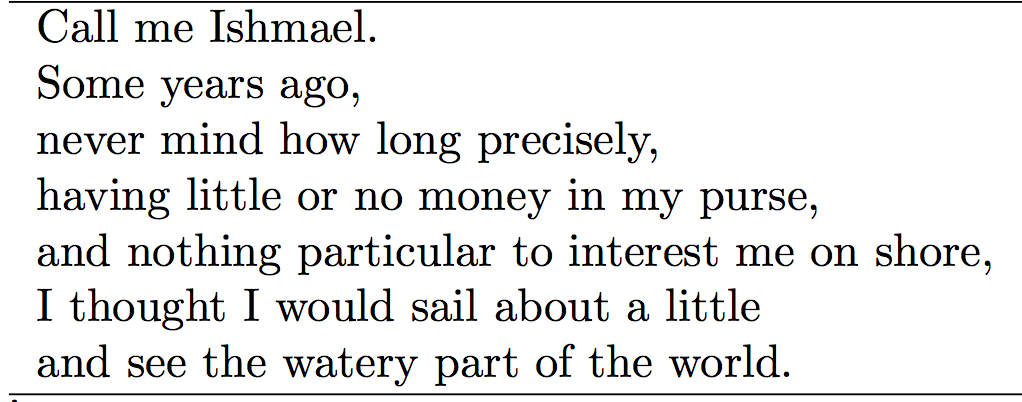
\includegraphics[width=7cm]{images/unbalanced} & \rightarrow &  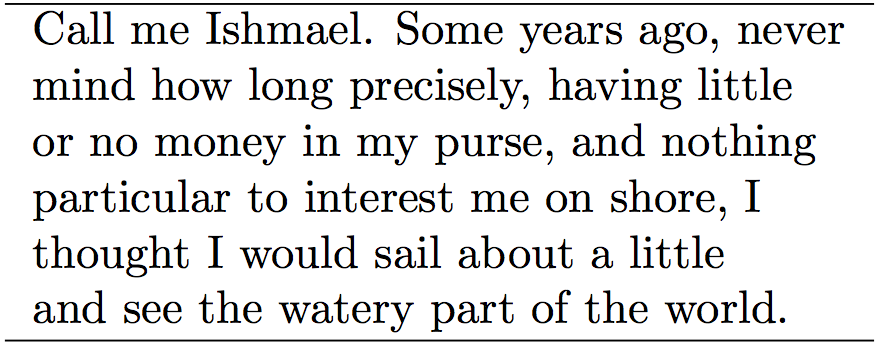
\includegraphics[width=7cm]{images/balanced}
			\end{tabular}
		\end{center}
		
	\hfil
	
	In order to accomplish this we will need to make use of dynamic programming. Here is the overview of how we will make use of this programming technique:
	
	\hfil
	
	\begin{itemize}
  		\item Find a recurrence relation for the optimal solution
  		\item Based on our recurrence relation, create an algorithm to solve our problem
	\end{itemize}
	
	
	\hfil


	\textbf{A: Recurrence Relation} \\
	
	In order to come up with a recurrence relation we need to understand what it is we are exactly computing. We are trying to re-arrange the text such that the "slack" or amount of spaces from the last word of every line are evenly distributed among the entirety of the text. This becomes a trivial task until we define what "even" means. Let us assume that "even" means to minimize the sum of all the "slacks". If we were to take this approach we would be left with several different viable solutions. See below for more details. Assume we have a max row width of 10.
	
	\hfil
	
		\begin{center}
			\begin{verbatim}
			                SOLUTION 1                             SOLUTION 2
			
				          Line  0123456789      Slack            Line  0123456789     Slack
				          ---------------------------            --------------------------
				           0    Ruelas      -->  4                0    Ruelas    -->   4
				           1    Juan is my  -->  0       VS       1    Juan is   -->   3
				           2    name        -->  6                2    my name   -->   3
				           		                    
				              4 + 0 + 6 = 10                         4 + 3 + 3 = 10                                     	
			\end{verbatim}				
		\end{center} 
		
		As you can see from the figure above, since we define "even" to be the minimization of all the slacks of every line, we will have multiple "optimal" solutions. This is a problem since we can reproduce identical slack summations with different text patterns and as we can visually see, the pattern on the right appears to be more "even" than the left one. Because of this, we will define "even" to mean the summation of all the $slacks^2$. This will enable us to be greedy with our spaces and will force us to minimize the amount of slack on $every$ line. Look below to see what I mean.
		
		\hfil
		
		
		\begin{center}
			\begin{tabular}{c c c}
			    \textbf{SOLUTION 1}: 4 + 0 + 6 = 10 & VS & $4^2$ + $0^2$ + $6^2$ = 52 \\
				\textbf{SOLUTION 2}: 4 + 3 + 3 = 10 & VS & $4^2$ + $3^2$ + $3^2$ = 34
			\end{tabular}
		\end{center}
		
		\hfil
		
		From this we can see that the optimal solution which minimizes the amount of slack on every line is the second solution. We will use this property of squaring the slack values to aid us in creating a recurrence relation. Essentially we will compute the minimum $slack^2$ for all combinations of words that fit within our row width (accounting for spaces where needed) and then find the "least cost slack" solution of each sub problem to determine our optimal solution for the pretty print. 
		
		\hfil
		
		
		\begin{center}
			\textbf{Recurrence Relation}: $OPT[n] = \displaystyle\min_{1\leq j \leq n} S^2_{i,n}+ OPT[j - 1])$
		\end{center}
		
		
		
	
	\hfil
	
	\textbf{B: The Algorithm} \\
	
	In order to begin the algorithm we need to understand what the recurrence relation itself is doing. It is returning to us the optimal solution on a subset of the word list $W$, and returns to us the least cost word arrangement which minimizes the amount of spaces used on a given line. We then use this to pre-compute all our values. Once we finish, we apply the same recurrence relation to our pre-computed values to find the optimal solution. We can break it down into 3 steps.  
	
	\begin{itemize}
		\item Given our word list $W$, we generate another array $A$ of equal length $L$, but instead of every value being a word, it will be the length of the word.
  		\item Generate a $slack^2$ matrix (accounting for spaces where needed) from $A$ of size $L \times L$ 
  		\item Find the optimal solutions to our sub problems, keeping track of each solution and "marking" our array for line breaks (aka our traceback)
	\end{itemize}
	
	\hfil
	
		Look at the pseudo code below
		
	\hfil	
	
	
	
	\definecolor{light-gray}{gray}{0.95}
	\lstset{columns=fullflexible, basicstyle=\ttfamily,backgroundcolor=\color{light-gray},xleftmargin=0.1cm,frame=lr,framesep=8pt,framerule=0pt}
    
    
	\begin{lstlisting}
	
		S = slack squared 2d matrix
		OPT[0] = 0
		#traverse the 2d array to find our traceback
		for k in range(0, len(S)):
			for j in range(0, len(S[k]):
				# find the optimal solution within a given row
				if (OPT[k] > ( S[j][k] + OPT[j - 1] )) :
					OPT[k] = S[j][k] + OPT[j - 1]
		
		return OPT[len(S)]
		
		 
	\end{lstlisting}
	
	\hfil
	

\end{solution}



\begin{solution} \textbf{Baby Faces v.s. Heels}\\

	This is a simple graph traversal problem that can be solved by running a BFS. Since we are given the number $n$ of professional wrestlers (nodes) a rivalry list $r$ (edges), we can create a graph $G$ by using the rivalry list to connect accordingly. Then we perform a BFS until we visit all vertices. Once we sort out the levels of connection, we can call all wrestlers who are on an even level "Babyfaces" and all wrestlers who are on an odd level "Heels". Once all wrestlers are assigned to their respective camps, we check each edge to verify that it only connects rivals. Because we know that a BFS has a O($V + E$) running time, we know that it will run in O($r + n$) time. 
	
	
	\hfil
	

	
\end{solution}

\end{document}









